\chapter{Infraestructura}\label{cap.infraestructura}
En este capítulo se describen los programas y dispositivos en los que nos hemos apoyado para la elaboración de este proyecto.
Debido a la naturaleza de la plataforma JdeRobot, el sistema operativo que se ha elegido para el desarrollo y ejecución de los componentes ha sido Linux (la distribución Ubuntu 16.04) y el lenguaje de programación Python (versión 2.7 para compatibilidad de JdeRobot con ROS-Kinetic).

\section{Parrot Ar.Drone 2}

Este es el drone que ha utilizado durante las pruebas reales. Parrot\footnote{https://www.parrot.com/global/} es un fabricante de dispositivos de diferente naturaleza, que van desde manos libres para teléfonos pasando por todo tipo de robots. Fue uno de los fabricantes que más popularizaron los drones a partir de 2010 con su primer Ar.Drone.

Este drone está dotado de una API de comunicaciones que forma parte de un SDK\footnote{http://developer.parrot.com/} que proporciona el fabricante de manera gratuita para obtener los datos de los sensores y/o control de los motores del cuadricóptero. Se ha utilizado la versión 2.4.

Posee dos cámaras, una ventral y otra frontal, incluye un acelerómetro y todo el procesado se realiza en un ARM de dos núcleos a bordo. Por último, está dotado de Wi-Fi como canal de comunicaciones por defecto y genera un punto de acceso sin contraseña para que los dispositivos se conecten y comuniquen con él. 

%%%%%%
%%%%%%\section{Interfaz Gráfica de usuario}
%%%%%%También conocida como \textit{GUI}, es el software encargado de simplificar la interacción con los usuarios. Proporciona texto, imágenes y diferentes objetos gráficos para representar la información y e interactuar con las acciones que se ofrezcan en un programa.

%%%%%%\subsection{Qt}
%%%%%%Qt\footnote{http://www.qt.io/} es una biblioteca multiplataforma cuyo objetivo principal es el de facilitar el diseño de interfaces gráficas de usuario. Su modelo de desarrollo es el de software libre y de Código Abierto, bajo la licencia GPL v3 y LGPL v2.1. Está programada en C++ , aunque puede ser utilizada junto a otros lenguajes de programación, como por ejemplo PyQt en Python. Ofrece un \textit{ambiente de desarrollo integrado}(IDE en inglés) llamado QtCreator, que facilita el proceso de desarrollo y el diseño gráfico del GUI. La versión utilizada en este proyecto es la 4.8.

%%%%%%\begin{figure}[H]
%%%%%%\centering
{%%%%%%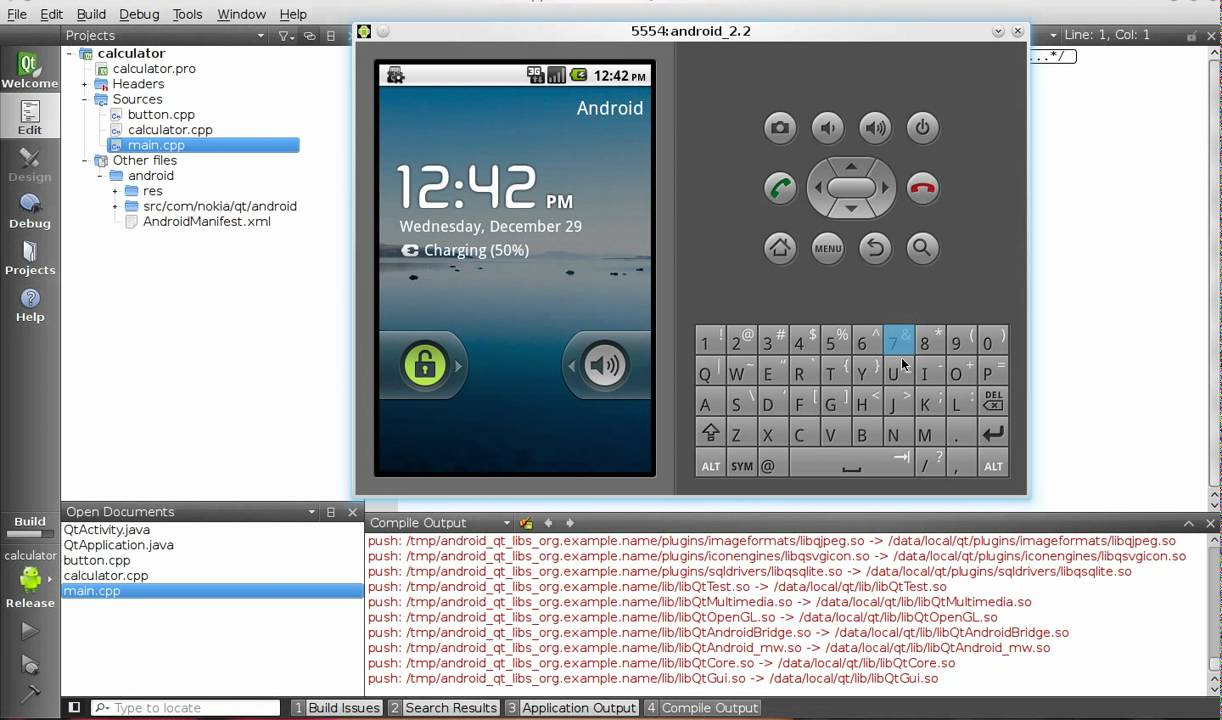
\includegraphics[scale=0.2]{imag/qt.jpg}}\hspace{10mm}
	%\subfloat[Personas en Gazebo]{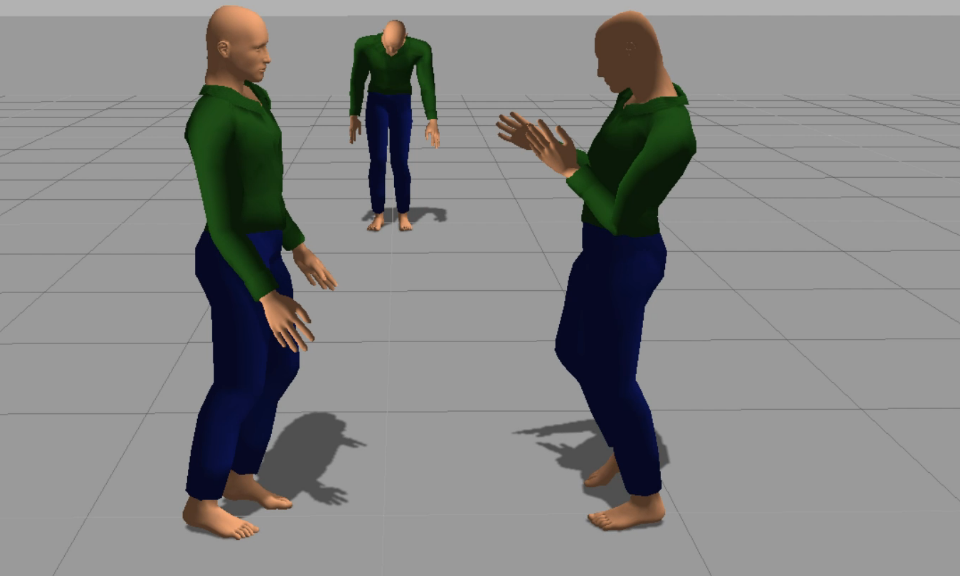
\includegraphics[scale=0.26]{imag/gazebo2.png}}
	%%%%%%\caption{Qt Creator}
	
	%%%%%%\label{FIG:31_qtcreator}
	%%%%%%\end{figure}
	
	%%%%%%\subsubsection{PyQt}
	
	%%%%%%PyQt\footnote{https://riverbankcomputing.com/software/pyqt/intro} es una colección de bibliotecas escritas en Python y C++ que complementan Qt. Mantiene la característica multiplataforma  y es un partner reconocido oficialmente por el propio Qt. Se encuentra bajo la licencia GPL v3 y la \textit{Riverbank Commercial License}. En este proyecto se ha utilizado para el desarrollo de componentes utilizando el lenguaje de programación Python. La versión utilizada en este proyecto es la PyQt5.
	
	\section{Intel Compute Stick}
	\label{sec:ics}
	
	Para dotar de autonomía y potencia de procesado al Ar.Drone 2, se ha decidido utilizar un co-procesador a bordo. Se ha utilizado este dispositivo Intel Compute Stick que entra dentro de la categoría de \textit{miniordenadores} u ordenadores de tamaño reducido. La principal ventaja es su relación peso y rendimiento, ya que está equipado con un procesador de dos núcleos, capaz de ejecutar 4 hilos simultáneamente. Cuenta con Wi-Fi integrado, además de un puerto USB, lector de tarjetas SD y HDMI como salido de vídeo.
	
	\begin{figure}[H]
		\centering
		\includegraphics[scale=0.6]{imag/ics.jpg}
		\caption{Imagen de Intel compute Stick}
		\label{FIG:34_ics}
	\end{figure}
	
	\section{Biblioteca OpenCV} \label{sec:opencvs}
	
	OpenCV\footnote{https://opencv.org/} es una biblioteca de visión artificial de código abierto, que tiene un conjunto de transformaciones y operaciones con imágenes o matrices que facilitan el procesamiento de las mismas. Es el estándar internacional de facto en procesamiento de imágenes. Está programada en C++ y Python y en este TFG se ha utilizado la versión 3.4.
	
	En este proyecto se ha utilizado para realizar filtros de color en imágenes para identificar la balizas de despegue y aterrizaje. Otro uso es para realizar transformaciones morfológicas en imágenes como la erosión y la dilatación, que permiten eliminar la sombra que proyecto el drone. Por último, de esta biblioteca también se han utilizado transformaciones geométricas de matrices para estimar la posición relativas del drone a partir de la información de balizas en una imagen de dos dimensiones.
	
	\section{Biblioteca AprilTags}
	\label{sec:AprilTags}
	
	En este proyecto se utilizará una librería de balizas visuales denominada \textit{AprilTags} \footnote{https://april.eecs.umich.edu/software/apriltag/}. Es un sistema de visualización fiduciaria. Estas balizas se basan es símbolos diseñados para ser fácilmente reconocidos del resto del entorno \ref{FIG:33_apriltag}. Puede detectar uno o varios símbolos en la misma imagen, además de proporcionar información como la identificación y posición de cada símbolo dentro de una imagen de cada uno. Es un sistema robusto cuyo funcionamiento es independiente del ángulo y diferentes situaciones de luminosidad en la imagen.
	
	\begin{figure}[H]
		\centering
		{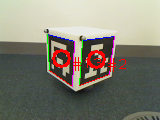
\includegraphics[scale=1.56]{imag/apriltag.png}}
		%\subfloat[Personas en Gazebo]{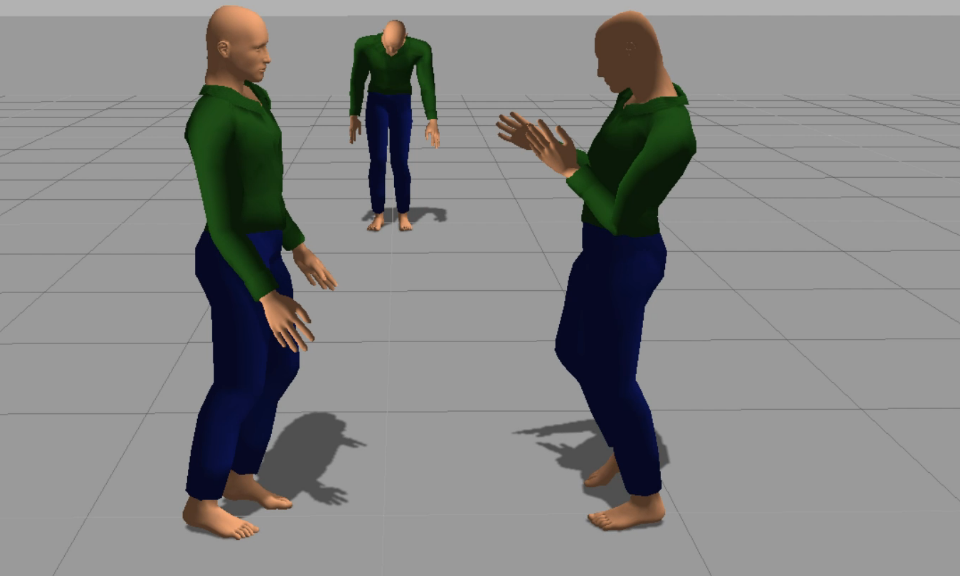
\includegraphics[scale=0.26]{imag/gazebo2.png}}
		\caption{Ejemplo de detección en AprilTag}
		
		\label{FIG:33_apriltag}
	\end{figure}
	
	
	Los símbolos se dividen en diferentes familias. Estas familias utilizan un número de bits y de distancia de Hamming predefinidos. Dentro de cada familia, se generan los diferentes símbolos, asignando un único ID o identificador. Esto permite el reconocimiento en caso de tener varias balizas al mismo tiempo en el campo de visión.
	
	Sus aplicaciones son muy variadas, desde la captura de movimiento en objetos hasta sistemas de navegación basada en balizas. Otra de sus aplicaciones es la de realidad aumentada, sustituyendo el símbolo por una imagen virtualizada.
	
	Además del sistema de balizas se proporciona una biblioteca que ofrece funciones de identificación de estas balizas en imágenes. Esta biblioteca está escrita en C y Java pero Ed Olson de Massachusetts Institute of Technology (MIT) ha creado una adaptación en C++. El código\footnote{https://svn.csail.mit.edu/apriltags} es abierto y está protegido bajo la LGPL v2.1. Entre sus dependencias se encuentran OpenCV y Eigen3, ambas son bibliotecas de tratamiento de imagen en Linux. A través de la utilización de un recubrimiento \footnote{https://github.com/swatbotics/AprilTag/toree/máster/Python} para Python ha sido posible su integración con la aplicación final de este TFG.
	
	\begin{figure}[H]
		\centering
		{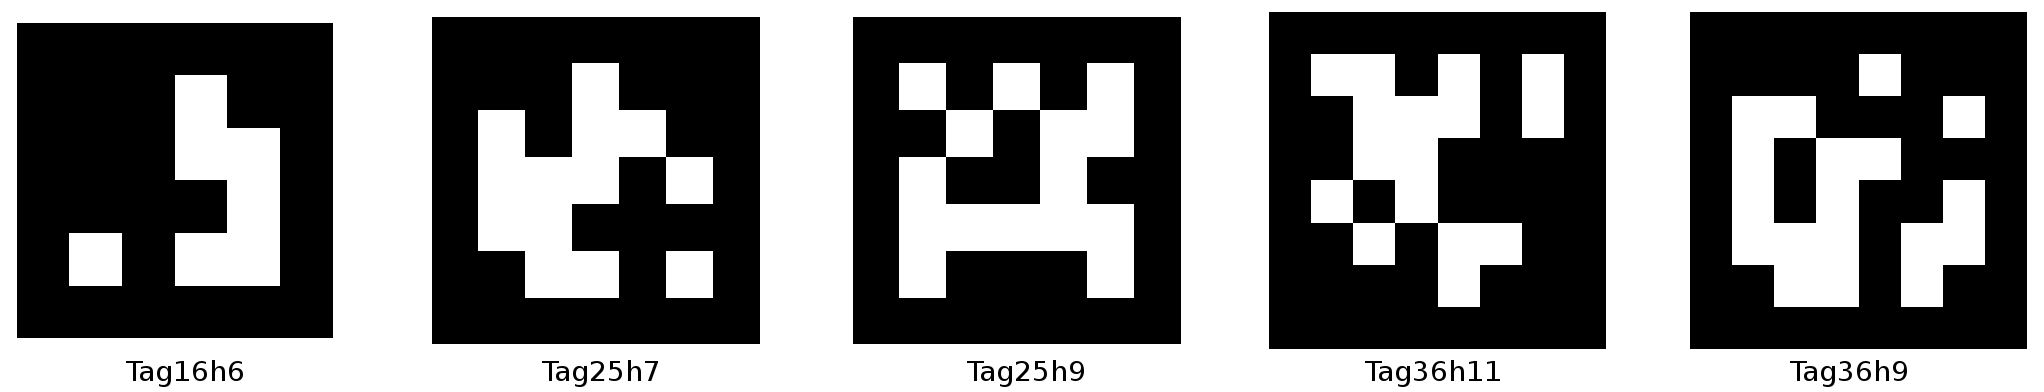
\includegraphics[scale=0.2]{imag/apriltags-codes.png}}
		%\subfloat[Personas en Gazebo]{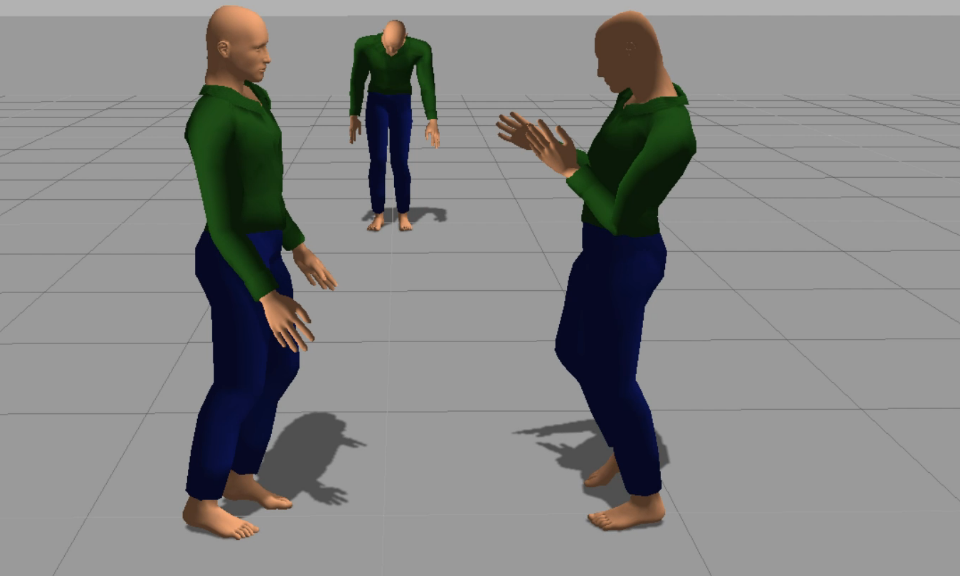
\includegraphics[scale=0.26]{imag/gazebo2.png}}
		\caption{Ejemplos de familias en AprilTag}
		
		\label{FIG:34_apriltag_families}
	\end{figure}
	
	
	\section{Entorno JdeRobot}
	\label{sec:Jderobot}
	
	En el mundo de la robótica existen diferentes plataformas que simplifican y aportan las herramientas necesario para el desarrollo de aplicaciones en robots. JdeRobot es una de ellas y consiste en una colección de drivers, herramientas y bibliotecas robóticas, domóticas y de visión artificial. Estas piezas de software están escritas en diferentes lenguajes como C++ o Python y su interoperación se realiza a través de interfaces ICE o interfaces ROS. En ella participan desarrolladores de diferentes niveles desde profesionales del sector, profesores, alumnos de la Universidad Rey Juan Carlos y de otras universidades internacionales. El código fuente es libre y está bajo la licencia GPL v3 y la documentación se encuentra protegido bajo la licencia de Creative Commons by-SA. La versión utilizada en este proyecto es la 5.6.4\footnote{https://github.com/JdeRobot}.
	
	Durante el desarrollo de este TFG, componentes de esta plataforma como \texttt{uav\_viewer}, \texttt{uav\_viewer\_py}, \texttt{slam\_markers} y \texttt{ardrone\_server} han servido de referencia y han tenido una gran relevancia para el aprendizaje de la plataforma.
	
	Se repasan a continuación los más relacionados con este trabajo:
	
	\subsection{Ardrone\_Server}
	
	Este componente fue desarrollado en el TFG de Alberto  Martín \cite{AlbertoMartin} y permite a partir de un protocolo basado en interfaces ICE el envío y lectura de comandos específicos del SDK del Ar.Drone 2.
	Como resultado, podemos modificar la velocidad de los motores para cambiar la posición del drone, recibir las imágenes de sus cámaras, envío de órdenes predeterminadas como el aterrizaje o despegue, recibir la información de sensores, etcétera.
	
	\begin{figure}[H]
		\centering
		{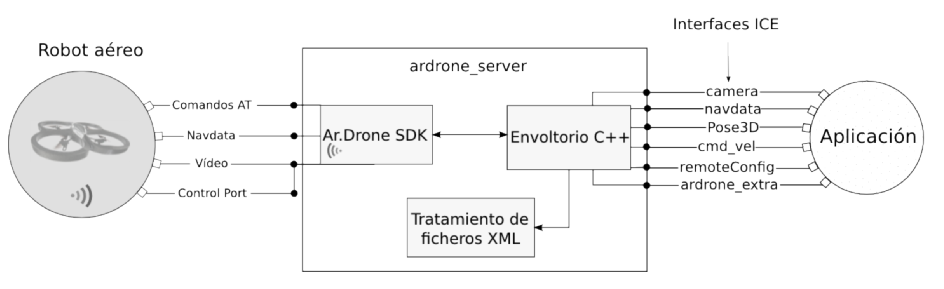
\includegraphics[scale=0.4]{imag/ardrone_server_structure.png}}
		\caption{Estructura de ardrone\_server}
		
		\label{FIG:32_ardrone_server}
	\end{figure}
	
	Está programado en C++ y es absolutamente necesario para cualquier comunicación con el drone real.
	
	
	
	\subsection{Teleoperadores uav\_viewer y uav\_viewer\_py} \label{subsec:uavviewer}
	
	Ambos son componentes de JdeRobot y ofrecen una GUI para enviar comandos tanto al cuadricóptero real, como al Ardrone simulado o mostrar la información de los sensores y cámaras. 
	Los comandos se envían a través de interfaces ICE al componente \texttt{ardrone\_server}, que los transforma a su vez en comandos para el SDK del Ar.Drone 2. La principal diferencia entre ambos es el lenguaje en el que han sido desarrollados: \texttt{uav\_viewer\_py  }está escrito en Python y ofrece un GUI más parecido a los mandos físicos de teleoperación de drones mientras que \texttt{uav\_viewer} \ref{FIG:11_uav_viewer} está en C++.
	
	\subsection{Herramienta Color Tuner}
	\label{subsec:colorTuner}
	Este componente facilita la configuración de filtros de color utilizando OpenCV. En su interfaz gráfica se selecciona el espacio de color que queremos utilizar, RGB, YUV y HSV, siendo esta última la utilizada por nuestras aplicaciones. Dentro de la aplicación, las ventanas \textit{Source image} y \textit{Filtered image} mostrarán la imagen recibida y su versión filtrada respectivamente. Para especificar los valores que se aplicarán para filtrar, se modifica la posición deslizadores o \textit{sliders} que representan los valores máximos y mínimos de H (\textit{hue} o tinte), S (saturación) y V (value o luminosidad).
	
	
	\begin{figure}[H]
		\centering
		{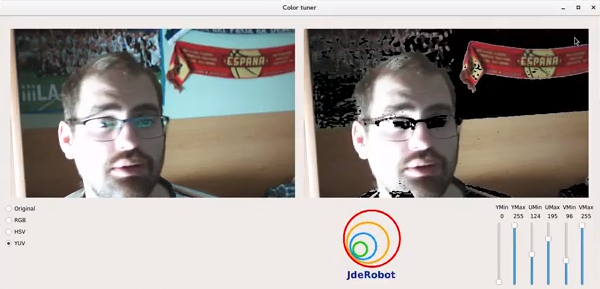
\includegraphics[scale=0.55]{imag/colortuner.png}}
		\caption{Ejemplo de Color Tuner aplicando filtros de color}
		
		\label{FIG:32_colorTuner}
	\end{figure}
	
	
	\subsection{Componente slam\_markers}
	\label{subsec:slam Markers}
	
	Esta herramienta permite mediante la aplicación de una serie de algoritmos de autolocalización basado en balizas visuales. Su algoritmo analiza las imágenes en 2D recibidas por la cámara y utiliza tanto la biblioteca OpenCV como AprilTags. Primero identifica si existen balizas \ref{FIG:32_slamMarkers} Una vez localizada, aplica funciones para calcular la posición y orientación en tres dimensiones de la cámara con respecto a la baliza. En el siguiente paso se ejecuta un proceso de fusión temporal y fusión espacial de la estimación obtenida. Por último, devuelve a través de una interfaz ICE las coordenadas 3D obtenidas como resultado de todo el proceso.
	 
	Ha sido desarrollada por Felipe Pérez en su TFM\footnote{http://jderobot.org/Flperez-tfm}. Ha sido programada en C++ y actualmente se encuentra aún en desarrollo. Para nuestro TFG se ha reimplementado su algoritmo en Python para facilitar la integración con la aplicación final y mejorar el rendimiento.
	
	\begin{figure}[H]
		\centering
		{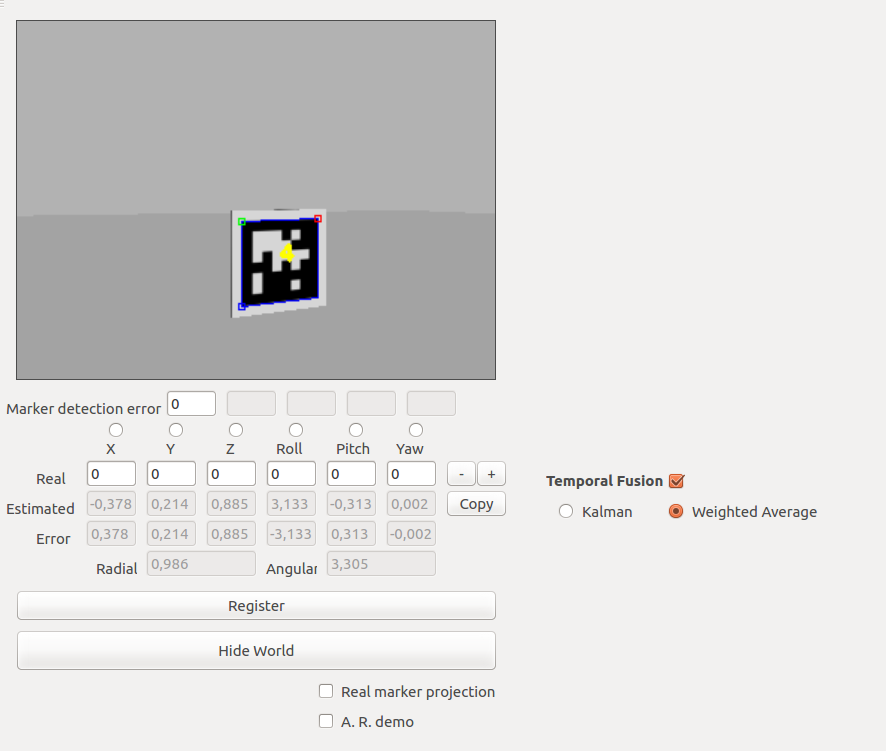
\includegraphics[scale=0.4]{imag/slam_markers_ui.png}}
		\caption{Ejemplo de slam\_markers identificando una baliza}
		
		\label{FIG:32_slamMarkers}
	\end{figure}
	
	
	\subsection{VisualStates}
	\label{subsec:VisualStates}
	
	Esta herramienta\footnote{http://jderobot.org/VisualStates} forma parte de la infraestructura JdeRobot  y su principal función es facilitar la creación de programas para robots basados en máquinas de estados finito con estados y transiciones. 
	
	Se caracteriza por tener una interfaz de usuario en la que podemos generar o modificar estados, teniendo siempre uno como principal a partir del cual comenzará la ejecución.
	Cada estado se compone por un código que será ejecutado en bucle hasta que se realice una transición a otro estado diferente. La herramienta genera como salida un programa que materializa el autómata, y que puede estar escrito tanto en Python como en C++.
	
	Las transiciones se dibujan entre los diferentes estados existentes especificando las condiciones temporales o basadas en variables que provocarán el cambio de estado.
	
	Adicionalmente proporciona un menú de configuración de interfaces ICE compatibles con JdeRobot, una sección de variables y funciones para que se compartan entre los diferentes estados. El menú también permite la modificación de la duración de las iteraciones periódicas en las que se van ejecutando los estados.
	
	Por último, tiene la capacidad de generar ejecutables y sus respectivos ficheros de configuración ICE. Esto facilita el empaquetado y el despliegue de los programas en un único fichero ejecutable.
	
	\begin{figure}[H]
		\centering
		{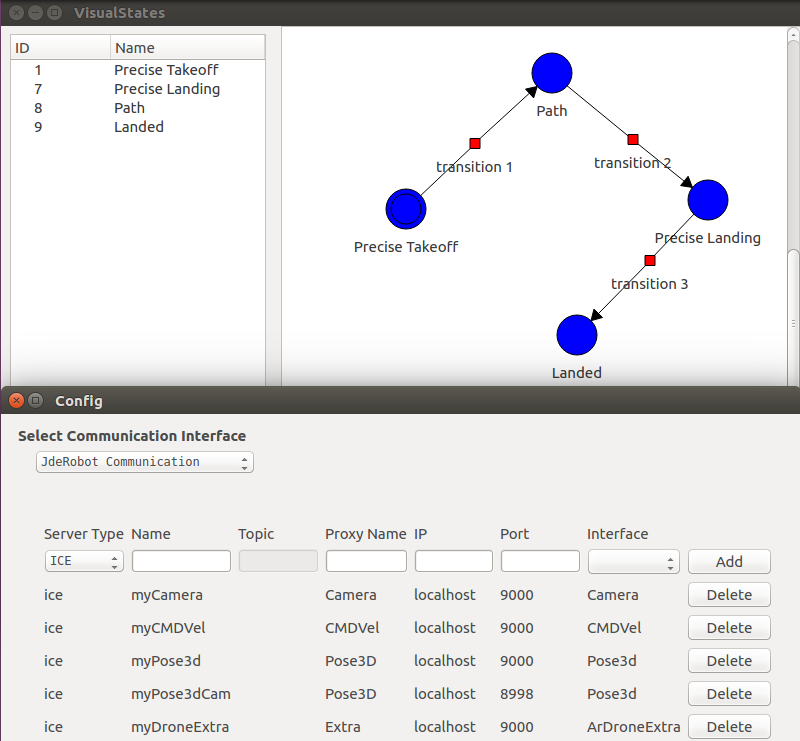
\includegraphics[scale=0.45]{imag/IMG32.png}}
		%\subfloat[Personas en Gazebo]{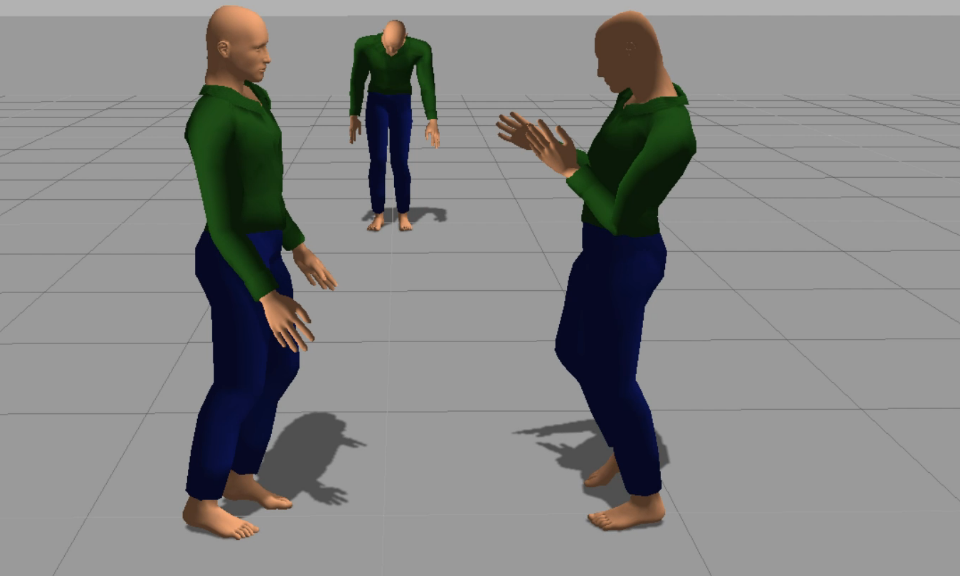
\includegraphics[scale=0.26]{imag/gazebo2.png}}
		\caption{Ejemplo de autómata generado con VisualStates}
		
		\label{FIG:33_visualstates}
	\end{figure} 
	
	\section{Bibliotecas ICE}
	
	ICE\footnote{https://zeroc.com/} es un \textit{middleware} de Código Abierto orientado a objetos que proporciona las herramientas, APIs y librerías necesarias para simplificar las comunicaciones entre componentes usando modelos basados en cliente y servidor y objectos distribuidos. En JdeRobot es la plataforma elegida como infraestructura para las comunicaciones entre nodos. Proporciona una capa transparente que se encarga de abrir y cerrar conexiones, la serialización de información, retransmisión de paquetes perdidos, etcétera. La versión utilizada en este proyecto es la 3.6
	
	\section{Simulador Gazebo}
	
	Este simulador de código abierto es la herramienta en la que se realizarán algunas las pruebas experimentales. En este TFG se ha utilizado la versión Gazebo 7.12 para simular al drone en diferentes escenarios. De este modo podremos evaluar previamente el código antes de ejecutarlo en el drone real. 
	Los escenarios simulados o mundos se crean con la propia aplicación y se definen con la extensión \textquotedblleft\texttt{.world}\textquotedblleft. Están escritos mediante SDF (\textit{Simulation Description Format}) que a su vez, está basado en el lenguaje XML y es muy popular en entornos de simuladores para robots.
	Estos mundos contienen modelos virtuales de robots que pueden tener un papel activo como un drone o pasivo como las balizas. El comportamiento activo se materializa mediante plugins que permiten la ejecución de código, interacciones con el motor de físicas del simulador, la obtención de imágenes desde cámaras virtuales, etcétera.
	
	\begin{figure}[H]
		\centering
		{\includegraphics[scale=0.3]{imag/gazebo-jackal-race.png}}
		\caption{Ejemplo de simulador Gazebo}
		\label{FIG:33_gazebo}
	\end{figure}
	
	%\section{OpenSSH} \label{sec:openssh}
	%Es una herramienta de código abierto para el acceso remoto a través de una autenticación utilizando el protocolo SSH \footnote{https://www.openssh.com/}. El tráfico se envía de forma cifrada para evitar que terceros puedan intervenir o escuchar el intercambio de información. Dispone de una variedad de opciones, métodos de autenticación y la capacidad de abrir túneles punto a punto de forma segura. En este TFG se ha utilizado su versión 7.7 y se ha empleado para intercambiar información entre el co-procesador y el ordenador desde el que queramos iniciar la aplicación final.